\chapter{Software}
\label{chapter:appsoft}
\thispagestyle{myheadings}

\graphicspath{{Appendix/Figures/}}


This appendix covers software architecture of the incoherent scatter radar (ISR) simulator that is in the code base. The simulator was developed to make synthetic data that one could use to create different processing algorithms and methods while having a known input or "truth" data. This simulator will take plasma fields of plasma parameters, create IQ from these parameters and then process that data to the point where it can estimate the input plasma parameters.

The need to create a full 3-dimensional software package was necessitated by the desire to explore the utility of the new phased array radar systems and their ability to measure 3-D fields of plasma parameters. This desire to understand the measurement capabilities of electronically scanned ISR lead to the following publication \cite{RDS:RDS20236} where this software package was used to create reconstructions of 3-D fields of plasma parameters.

The software itself has been developed in such a way that the code mirrors the processing. Overall there are three main classes: 

\begin{itemize} 
\item IonoContainer - A container class that holds information on the ionosphere or auto correlation functions (ACFs)/spectrums, both intrinsic and estimated.

\item RadarDataFile - A class that holds and operates on the radar data to create estimates of the autocorrelation function. The class takes files containing ISR spectrums and then creates ISR data and as a final step outputs instances of the IonoContainer class that holds estimates of the plasma ACF.

\item FitterMethodsGen - A class that applies the fitter to the data and outputs an instance of IonoContainer with the measured parameters. 
\end{itemize}

The overall flow can be seen in figure \ref{fig:swflow}, where  $\Theta$ is the plasma parameters $ g(\Theta)$ is a function that turns the plasma parameters to ISR spectrums, $ \mathbf{r}$ is the spectrums/ACFs for each point of time and space, $ \mathbf{Lr}$ is the radar's operator on the spectrums/ACFs, $ \rho$ is the measured ACFs from the radar and lastly $ \hat{\Theta}$ is the estimates of plasma parameters from $ \rho$ after least squares fitting.

\begin{figure}[!h]
\centering
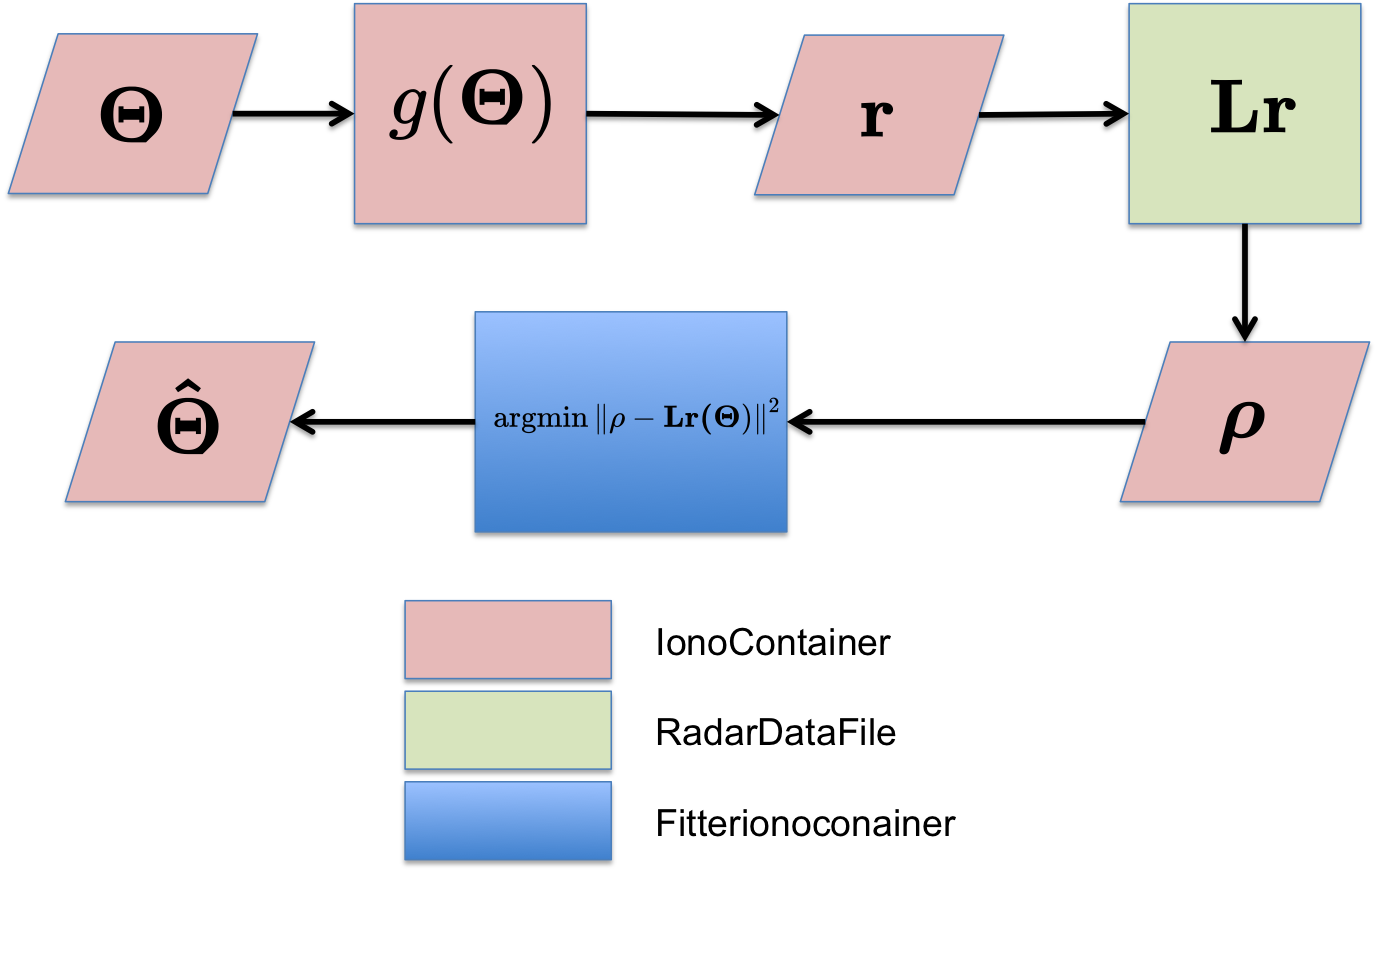
\includegraphics[width=6.0in]{softwareflowandmath}
% where an .eps filename suffix will be assumed under latex, 
% and a .pdf suffix will be assumed for pdflatex; or what has been declared
% via \DeclareGraphicsExtensions.
\caption{Software flow diagram}
\label{fig:swflow}
\end{figure}

This report is broken up in to the following chapters. The next chapter will cover the method to calculate the ISR spectrum. There are a number of publications on this including \cite{dougherty:farley1960, hagfors1971, sheffield2010} that cover this area but we focus on the treatment found in \cite{kudeki:milla:1}. Next the method to form the ISR data will be shown, this will include the signal processing steps taken to create the data. The processing of the data from estimating the lags to fitting the plasma parameters will then be covered. We will focus on methods for long pulse but we will show where this differentiates when using other waveforms such as alternating codes and Barker codes. Lastly we will show examples of the output of the ISR simulator at a number of different spots in the processing chain.